\chapter{
تصویر تصادفی پایدار
}

روش تصویر تصادفی پایدار
\LTRfootnote{Stable Random Projections}
\cite{litez116, litez166, litez19, litez99, litez96, litez104}
یک روش پرکاربرد در داده‌کاوی و یادگیری ماشین است. با این روش به طور کار 
$l_\alpha (0 < \alpha \leq 2)$
فاصله در داده‌های حجیم (برای مثال: وب یا جریان‌های داده‌ی حجیم) محاسبه می‌شود. در این روش حافظه‌ی کمی استفاده شده و فقط یک بار پایش داده‌ها کافی است. 

\begin{figure}[h]
\centering
\begin{latin}
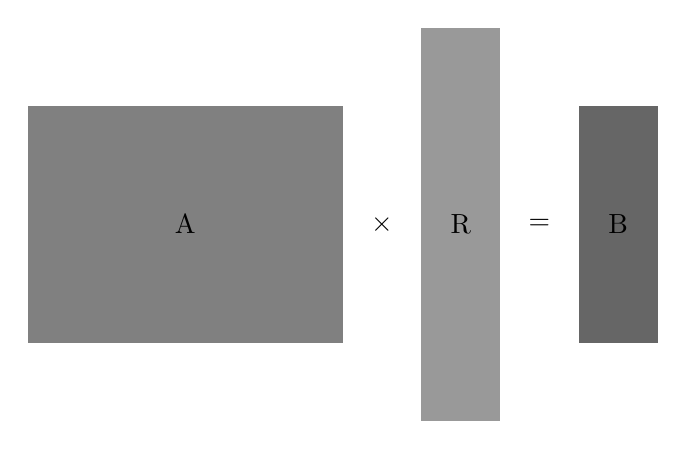
\begin{tikzpicture}
\fill[black!50!white] (0,1) rectangle (4,4);
\node at (2,2.5) [rectangle,preaction={fill=black!50},font={A}] {};
\node at (4.5,2.5) [rectangle,preaction={fill=black!0},font={$\times$}] {};
\fill[black!40!white] (5,0) rectangle (6,5);
\node at (5.5,2.5) [rectangle,preaction={fill=black!40},font={R}] {};
\node at (6.5,2.5) [rectangle,preaction={fill=black!0},font={=}] {};
\fill[black!60!white] (7,1) rectangle (8,4);
\node at (7.5,2.5) [rectangle,preaction={fill=black!60},font={B}] {};
\end{tikzpicture}
\end{latin}
\caption{
روش تصویر تصافی پایدار ماتریس داده‌ی 
$\mathbf{A} \in \mathbb{R}^{n \times D}$
را در یک ماتریس تصادفی
$\mathbf{R} \in \mathbb{R}^{D \times k}$
ضرب می‌کند تا ماتریس تصویر شده‌ی 
$\mathbf{B} = \mathbf{AR} \in \mathbb{R}^{n \times k}$
حاصل شود.
}
\label{fig:randomprojection}
\end{figure}

همانطور که در 
\autoref{fig:randomprojection}
می‌بینید.
